\documentclass[a4paper, 11pt]{article}
\usepackage[utf8]{inputenc}
\usepackage[T1]{fontenc}

\usepackage[margin=1in]{geometry}
\usepackage{amsmath, amsfonts, amsthm, amssymb, amsxtra}

\usepackage{graphicx}
\usepackage{float}

\usepackage[dvipsnames]{xcolor}

\usepackage{tabularray}
\usepackage{enumitem}
\usepackage{multicol}

\usepackage{hyperref}
\hypersetup{hidelinks}

\usepackage{tikz}
\usetikzlibrary{intersections, angles, calc, positioning}
\usetikzlibrary{shapes.geometric, arrows.meta}
\usetikzlibrary{decorations.pathmorphing, decorations.pathreplacing}

\setlength{\parindent}{0pt}
\setlength{\parskip}{5pt}

\makeatletter
\newcommand{\type}[1]{\def\@type{#1}}

\renewcommand*{\maketitle}{%
\vspace{-0.5cm}
\begin{tikzpicture}[remember picture, overlay]
    \node[anchor=south, align=center] (date) at ($(current page.north) + (0,-110pt)$) {\@date};
    \node[anchor=south, align=center, font=\itshape] (author) at (date.north) {\@author};
    \node[above=10pt of author, align=center, font=\scshape] (type) {\@type};
    \node[anchor=south, align=center, font=\bfseries\large] (title) at (type.north) {\@title};
    \node[anchor=west] (logo) at ($(current page.north west) + (\Gm@lmargin, -65pt)$) {
\includegraphics[height=3.15cm]{ufs_vertical_positiva.eps}};
    \draw ($(current page.north west) + (\Gm@lmargin, -120pt)$) -- ($(current page.north east) + (-\Gm@lmargin, -120pt)$);
\end{tikzpicture}
\vspace{45pt}
}%
\makeatother

\usepackage{notomath}

\definecolor{azulfundo}{RGB}{51, 149, 255}
\definecolor{cinzaborda}{RGB}{66, 73, 80}
\definecolor{bicoum}{RGB}{181, 141, 57}
\definecolor{bicodois}{RGB}{206, 157, 56}
\definecolor{novo}{RGB}{108, 107, 91}

\title{EFEITO BLUR EM\\IMAGENS .ppm}
\type{Atividade}
\author{Bruno Sant'Anna}
\date{\today}

\begin{document}
\maketitle

\section*{Introdução}
Uma \textit{convolução} é uma operação matemática com muitas utilidades, inclusive em computação gráfica e processamento de imagens.
Por meio de um \textit{kernel de convolução}, que é uma matriz pequena com uma série de pesos, que mudam o valor de um pixel na imagem dependendo dos valores dos pixels ao seu redor.
Nesse caso para aplicar um efeito de \textit{blur}, estaremos usando um kernel onde a soma de todos os pesos é igual a 1, por exemplo
\begin{equation}\label{eq:uniform}
    \begin{pmatrix}
        \frac{1}{9} & \frac{1}{9} & \frac{1}{9}\\[5pt]
        \frac{1}{9} & \frac{1}{9} & \frac{1}{9}\\[5pt]
        \frac{1}{9} & \frac{1}{9} & \frac{1}{9}
    \end{pmatrix}
\end{equation}

\begin{equation}\label{eq:gaussian}
    \begin{pmatrix}
        0.003 & 0.013 & 0.022 & 0.013 & 0.003\\
        0.013 & 0.060 & 0.098 & 0.060 & 0.013\\
        0.022 & 0.098 & 0.162 & 0.098 & 0.022\\
        0.013 & 0.060 & 0.098 & 0.060 & 0.013\\
        0.003 & 0.013 & 0.022 & 0.013 & 0.003
    \end{pmatrix}
\end{equation}

\section*{Funcionamento}

De forma simplificada, quando aplicamos um kernel em uma imagem, para cada pixel $(i,j)$ da imagem o kernel é posicionado com o seu centro em $(i,j)$ e multiplicamos o cada coordenada da imagem com a coordenada do kernel sobreposto e somamos, esse é o valor do pixel $(i,j)$ na imagem nova.
Vale lembrar que cada pixel da imagem colorida é um vetor de $\mathbb{N}^3$ onde cada entrada varia de 0 a 255, a primeira entrada é o canal de cor vermelho, a segunda verde e a terceira azul, conhecido como sistema RGB.

Usando o kernel \ref{eq:uniform} como exemplo:


\begin{center}
    \begin{minipage}{0.4\textwidth}
        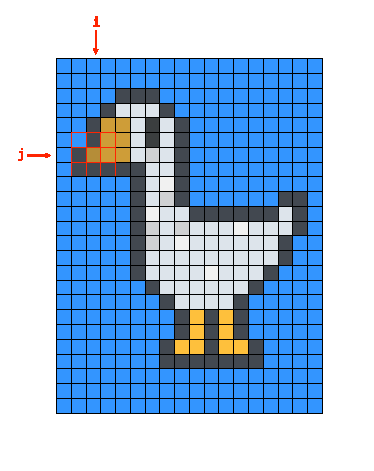
\includegraphics[height=7.5cm]{goose.pdf}
    \end{minipage}
    \begin{minipage}{0.55\textwidth}
        $
        \left\lfloor
        \textcolor{azulfundo}{\frac{1}{9} \blacksquare} +
        \textcolor{cinzaborda}{\frac{1}{9} \blacksquare} +
        \textcolor{bicodois}{\frac{1}{9} \blacksquare} +
        \textcolor{cinzaborda}{\frac{1}{9} \blacksquare} + 
        \textcolor{bicoum}{\frac{1}{9} \blacksquare} + 
        \textcolor{bicodois}{\frac{1}{9} \blacksquare} +
        \textcolor{cinzaborda}{\frac{1}{9} \blacksquare} + 
        \textcolor{cinzaborda}{\frac{1}{9} \blacksquare} + 
        \textcolor{cinzaborda}{\frac{1}{9} \blacksquare}
        \right\rfloor  = \textcolor{novo}{\blacksquare}
        $
    \end{minipage}
\end{center}

Ou com a notação vetorial

$\big\lfloor
\frac{1}{9} (\textcolor{red}{51}, \textcolor{green}{149}, \textcolor{blue}{255}) + 
\frac{1}{9} (\textcolor{red}{66}, \textcolor{green}{73}, \textcolor{blue}{80}) + 
\frac{1}{9} (\textcolor{red}{206}, \textcolor{green}{157}, \textcolor{blue}{56}) + 
\frac{1}{9} (\textcolor{red}{66}, \textcolor{green}{73}, \textcolor{blue}{80}) + 
\frac{1}{9} (\textcolor{red}{181}, \textcolor{green}{141}, \textcolor{blue}{57}) +
\frac{1}{9} (\textcolor{red}{206}, \textcolor{green}{157}, \textcolor{blue}{56}) + 
$\\[3pt]
$\textcolor{white}{\big\lfloor} 
\frac{1}{9} (\textcolor{red}{66}, \textcolor{green}{73}, \textcolor{blue}{80}) + 
\frac{1}{9} (\textcolor{red}{66}, \textcolor{green}{73}, \textcolor{blue}{80}) + 
\frac{1}{9} (\textcolor{red}{66}, \textcolor{green}{73}, \textcolor{blue}{80})
\big\rfloor = 
(\textcolor{red}{108}, \textcolor{green}{107}, \textcolor{blue}{91})
$


\section*{Resultados}
% first blurred goose image
% then unblurred turtle
% kernel 3x3
% kernel 5x5
% 7x7
% 9x9
% gaussian

% make table 3x2 with caption

% extra kernel (edge detection)




\end{document}